\chapter[Quantum States]{Quantum States}
\label{sec:2_quantum_states}


\chaptermark{Quantum States}

\rdv{Cleaned up, except for the duplicate introduction of ket.  It's still tempting to rewrite whole chunks of this chapter.}


In this chapter, we will learn about quantum states: how to write them down, what they represent, and how they differ from classical states.
Then, we will learn how to operate on and extract information from quantum states using unitary operations and measurements.
Lastly, we will discuss multiple quantum states and how to describe them. 
Most of this chapter will be familiar to those who have taken an introductory quantum computing course.

\section{Qubits}

% \subsection*{2.1.1: Qubits (Quantum bit)}

% Recall from Chapter 1 that all information can be represented by classical bits in the classical world. Classical bits are confined to either the zero or one states, whereas the qubit can be "in-between" zero or one in  \textbf{\emph{superposition}}\index{superposition} states. Mathematically, the general qubit state for a superposition of $\ket{0}$ and $\ket{1}$ is represented using notation known as \textbf{\emph{Dirac Notation}}, written
% \begin{equation}
% \ket{\psi} = \alpha \ket{0} + \beta\ket{1} 
% \end{equation}
%  where $\ket{\cdot}$ is pronounced \emph{ket}, $\psi$ (\emph{psi}) represents a general qubit state, $\alpha,\beta \in \mathbb{C}$.\label{def:ket}




First, let's discuss quantum bits, also known as \textbf{\emph{qubits}}\index{qubit}. We have seen in the previous chapter that information can be represented by classical bits. In the classical world, a classical bit can only be in two states: it can be in a state we label \emph{zero}, or in a state we label \emph{one}, nothing in between. In contrast, a quantum bit can be anything in between. It can be 100\% zero or 100\% one, but it can also be 50\% zero and 50\% one or 1\% zero and 99\% one. Such a state is called a \textbf{\emph{superposition}}\index{superposition} of zero and one. It's not that we don't know what the state is, it really is neither zero nor one but it's somewhere in between. (This notion of "in between" is not a completely accurate description, but it will do for now.  As we do the mathematics over the next several sections, your understanding will grow.)

% Dirac Notation w/ annotation
\begin{figure}[H]
    \centering
    % \includegraphics[width=0.8\textwidth]{lesson2/dirac_notation.pdf}
    % \includegraphics[width=1\textwidth]{lesson2/R2L2fig1.pdf}
    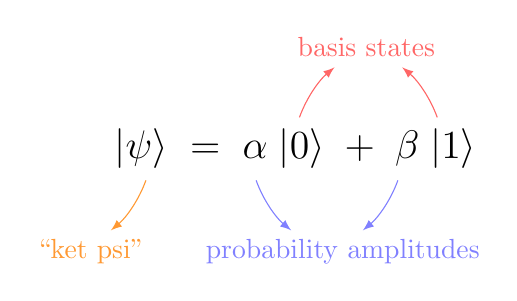
\begin{tikzpicture}
    \node[] at (0,0) {\Large $|\psi\rangle \; = \; \alpha \; |0\rangle \; + \; \beta \; |1\rangle$};
    
    \draw[-latex,red!60] (0.05,0.4) arc[start angle=160, end angle=130, radius=1.5];
    \draw[-latex,red!60] (1.8,0.4) arc[start angle=20, end angle=50, radius=1.5];
    \node[red!60] at (0.9,1.3) {basis states};

    \draw[-latex,blue!50] (-0.5,-0.4) arc[start angle=200, end angle=230, radius=1.5];
    \draw[-latex,blue!50] (1.3,-0.4) arc[start angle=340, end angle=310, radius=1.5];
    \node[blue!50] at (0.6,-1.3) {probability amplitudes};

    \draw[-latex,orange!80] (-1.9,-0.4) arc[start angle=340, end angle=310, radius=1.5];
    \node[orange!80] at (-2.6,-1.3) {``ket psi''};
    \end{tikzpicture}
    
    \caption[Dirac ket notation.]{Breakdown of the Dirac ket notation.}
    \label{fig:ket-notation}
\end{figure}

The most common notation for writing down the state of a qubit (or more than one qubit) is called the \textbf{\emph{Dirac notation}}\index{Dirac notation}, and it's extremely useful.
A general superposition of a qubit can be written as pictured in Fig.~\ref{fig:ket-notation}.
The funny angle bracket \ket{\cdot} is called a \textbf{\emph{ket}}\index{ket}. The symbol $\psi$ (Greek letter ``psi'') in a ket, which we will call ``state psi'' or ``ket psi'' interchangeably, is often used to describe a general state of a qubit. $\ket{0}$ and $\ket{1}$ are called the \textbf{\emph{basis states}}\index{basis states}, and they determine what our state is. This $\alpha$ and $\beta$ are \textbf{\emph{probability amplitudes}}\index{probability amplitudes} that tell us how much of the state is in zero and how much of the state is in one.  These probability amplitudes can be any complex numbers, provided that they satisfy the following normalization condition,
\begin{align}
    |\alpha|^2 + |\beta|^2 = 1.
    \label{eq:normalization-condition}
\end{align}
It should be read as ``mod alpha squared plus mod beta squared is equal to one''. This condition ensures that whatever measurements we do in the future on this state produce results with the correct probabilities.


% Bloch Sphere
\begin{figure}[H]
    \centering
    %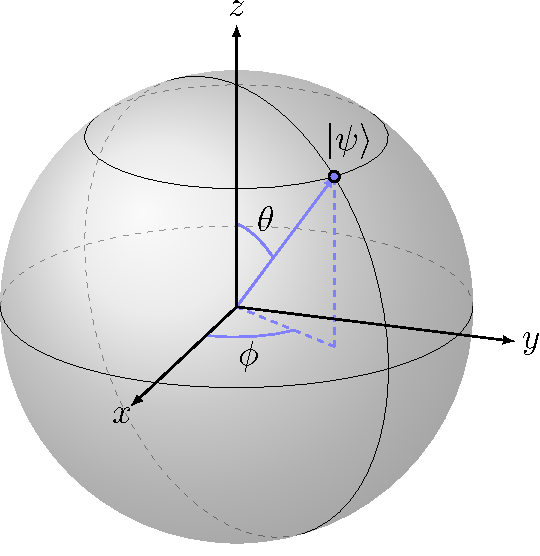
\includegraphics[width=0.5\textwidth]{lesson2/bloch_sphere.pdf}
    \def\r{4}
    \tdplotsetmaincoords{70}{115}
    \def\azimuthP{40}
    \def\polarP{60}
    \def\circleSize{88.5}
    
    \begin{tikzpicture}[tdplot_main_coords,scale=0.7,every node/.style={scale=0.7}]

        \tdplotsetcoord{O}{0}{0}{0}
        \tdplotsetcoord{P}{\r}{\azimuthP}{\polarP}
        \tdplotsetcoord{Q}{\r*sin(\azimuthP)}{90}{\polarP}

        \shade[tdplot_screen_coords,ball color=gray!40,opacity=0.5] (0,0,0) circle (\r);    % sphere
        \tdplotCsDrawLonCircle[tdplotCsBack/.style={black!50,dashed},thin]{\r}{\polarP-90}
        \tdplotCsDrawLatCircle[tdplotCsBack/.style={black!50,dashed},thin]{\r}{90-\azimuthP}
        \tdplotCsDrawLatCircle[tdplotCsBack/.style={black!50,dashed}]{\r}{0}

        \draw[-,blue!50,thick] (0:0.5*\r) arc (0:\polarP:0.5*\r);
        \node[] at ({0.4*\polarP}:0.27*\r) {\Large $\phi$};
        \tdplotsetthetaplanecoords{\polarP}
        \draw[tdplot_rotated_coords,-,blue!50,thick] (0:0.4*\r) arc (0:\azimuthP:0.4*\r);
        \node[tdplot_rotated_coords] at ({0.5*\azimuthP}:0.27*\r) {\Large $\theta$};

        \draw[-latex,thick] (O) -- (1.3*\r,0,0) node[pos=1.15] {\Large $x$};
        \draw[-latex,thick] (O) -- (0,1.3*\r,0) node[pos=1.07] {\Large $y$};
        \draw[-latex,thick] (O) -- (0,0,1.3*\r) node[pos=1.06] {\Large $z$};
        \draw[dashed,black!50] (O) -- (-\r,0,0);
        \draw[dashed,black!50] (O) -- (0,-\r,0);
        \draw[dashed,black!50] (O) -- (0,0,-\r);
    
        \draw[-latex,thick,blue!50] (O) -- (P);
        \draw[thick,dashed,blue!50] (O) -- (Q) -- (P);
    
        \tdplotCsDrawCircle[tdplotCsFill/.style=blue!50,thick]{\r}{\polarP}{\azimuthP}{\circleSize}
        \node[] at (4, 3.8, 4.7) {\Large $|\psi\rangle$};
    \end{tikzpicture}
    \caption[Bloch sphere.]{Bloch sphere visualization of a pure state $|\psi\rangle$.}
    \label{fig:bloch}
\end{figure}

Another very useful representation of quantum states is using the \textbf{\emph{Bloch sphere}}\index{Bloch sphere}, as shown in Figs.~\ref{fig:bloch} and \ref{fig:annotated-bloch}. This visual representation gives us a very intuitive way of thinking about quantum states. All the states are given as points on the surface of the sphere, parameterized by the angle $\theta$ and the angle $\phi$. Then the state $\ket{\psi}$ can be written in the following form,
\begin{equation}
|\psi\rangle=\cos \frac{\theta}{2}|0\rangle+e^{i \phi} \sin \frac{\theta}{2}|1\rangle
\end{equation}
where the probability amplitude for basis state 0 is given by $\cos(\theta/2)$ and the probability amplitude for basis state 1 is given by $\sin(\theta/2)$, multiplied by $e^{i \phi}$, known as the complex phase of the state. This phase does not affect the probability of finding a one when we measure the qubit, but it is critically important as part of the state and in quantum algorithms.

This \ket{\psi} is a general state, but let's look at some examples, as in Fig.~\ref{fig:annotated-bloch}. We have already encountered \ket{0} and \ket{1}, and they sit at the north and the south pole of the Bloch sphere, respectively. We also said that we can have an arbitrary superposition of zero and one. For example, we can have a state known as the \textbf{\emph{plus state}}\index{plus state}, written \ket{+}, which is an equal superposition of zero and one. The plus state appears on the equator of the Bloch sphere, at the point where the sphere's positive $X$ axis intersects the surface. We can have its friend the \textbf{\emph{minus state}}\index{minus state}, written \ket{-}, on the other side of the Bloch sphere. It also is an equal superposition, but this time it's on the negative side of the $X$ axis.  If you think about a rotation about the $Z$ along the equator, since $e^{i\pi} = -1$, it has the complex phase $\pi$.  We can also have two states on the $Y$ axis. One is called the ``plus i'' state, written \ket{i} or occasionally \ket{+i}, and the other is called ``minus i'', written \ket{-i}. You can see that again, both of these states are an equal superposition of zero and one, but this time the phase between zero and one is given by the complex number $i$ or the angle $\pi/2$ for \ket{i} and $-i$ or the angle $3\pi/2$ for \ket{-}.  Summarizing, these states are
\begin{equation}
    |\pm\rangle=\frac{1}{\sqrt{2}}(|0\rangle \pm|1\rangle), \qquad|\pm i\rangle=\frac{1}{\sqrt{2}}(|0\rangle \pm i|1\rangle).
\end{equation}

% insert Bloch sphere w/ axes labelled and |+> |-> meanings
\begin{figure}[H]
    \centering
    \def\r{4}
    \def\circleSize{88.5}
    \tdplotsetmaincoords{70}{115}
    \begin{tikzpicture}[tdplot_main_coords,scale=0.7,every node/.style={scale=0.7}]

        \tdplotsetcoord{O}{0}{0}{0}

        \shade[tdplot_screen_coords,ball color=gray!40,opacity=0.5] (0,0,0) circle (\r);    % sphere
        \tdplotCsDrawLonCircle[tdplotCsBack/.style={black!50,dashed},thin]{\r}{0}
        \tdplotCsDrawLonCircle[tdplotCsBack/.style={black!50,dashed},thin]{\r}{90}
        \tdplotCsDrawLatCircle[tdplotCsBack/.style={black!50,dashed}]{\r}{0}

        \draw[thick] (O) -- (\r,0,0);
        \draw[thick] (O) -- (0,\r,0);
        \draw[thick] (O) -- (0,0,\r);
        \tdplotCsDrawCircle[tdplotCsFill/.style=blue!50,thick]{\r}{0}{0}{\circleSize}
        \tdplotCsDrawCircle[tdplotCsFill/.style=blue!50,tdplotCsBack/.style={-},thick]{\r}{0}{0}{-88.8}
        \tdplotCsDrawCircle[tdplotCsFill/.style=blue!50,thick]{\r}{0}{90}{\circleSize}
        \tdplotCsDrawCircle[tdplotCsFill/.style=blue!50,tdplotCsBack/.style={-},thick]{\r}{0}{90}{-\circleSize}
        \tdplotCsDrawCircle[tdplotCsFill/.style=blue!50,thick]{\r}{90}{90}{\circleSize}
        \tdplotCsDrawCircle[tdplotCsFill/.style=blue!50,tdplotCsBack/.style={-},thick]{\r}{90}{90}{-\circleSize}
        \draw[dashed,black!50] (O) -- (-\r,0,0);
        \draw[dashed,black!50] (O) -- (0,-\r,0);
        \draw[dashed,black!50] (O) -- (0,0,-\r);
        \draw[-latex,thick] (\r,0,0) -- (1.3*\r,0,0) node[pos=1.5] {\Large $x$};
        \draw[-latex,thick] (0,\r,0) -- (0,1.3*\r,0) node[pos=1.4] {\Large $y$};
        \draw[-latex,thick] (0,0,\r) -- (0,0,1.3*\r) node[pos=1.38] {\Large $z$};
    
        \node[] at (\r,0.5,-0.4) {\Large $|+\rangle$};
        \node[] at (-\r,0.5,0.4) {\Large $|-\rangle$};
        \node[] at (0,\r+0.4,-0.4) {\Large $|i\rangle$};
        \node[] at (0,-\r-0.7,0.2) {\Large $|-i\rangle$};
        \node[] at (0,0.35,\r+0.6) {\Large $|0\rangle$};
        \node[] at (0,0.35,-\r-0.6) {\Large $|1\rangle$};
    \end{tikzpicture}
    \caption{Bloch sphere with $x$, $y$, and $z$ axis basis states.}
    \label{fig:annotated-bloch}
\end{figure}

\section{Unitary Operations}
\label{sec:2-2_unitary_operations}


% Classical (SSD) VS Quantum (Ion Trap)
\begin{figure}[H]
    \centering
    \includegraphics[width=0.9\textwidth]{lesson2/2-2_classical_quantum_info.pdf}
        \caption[Physical information-processing systems]{Examples of physical systems processing classical and quantum information.}
    \label{fig:physical-system}
\end{figure}

Let's see how we can manipulate quantum states, and therefore manipulate quantum information as well. We're going to do this with \emph{unitary operations}. One thing that you have to realize is that \emph{information is physical} (an aphorism coined by Rolf Landauer of IBM). This is because the information is represented by physical systems. Therefore, to change the information and process it, we have to interact with the physical systems that carry the information. In classical information, of course the primary processing technology is transistors manufactured using a photolithography process.  Computational states are represented using electrical charge, and information processing is done by using charge to control whether a switch is on or off, allowing charge to move from place to place within a computer chip.  Another very good example is HDDs (hard disk drives), where you read, write and manipulate information with very weak and precise magnetic fields. For an example of a younger technology, we can look at the "solid-state drive" where you do the same thing, but you achieve it by manipulating very weak electric currents.

In quantum information, on the other hand, we have physical systems such as \textbf{\emph{ion traps}}\index{ion traps}, from companies such as IonQ and Quantinuum. The atoms are suspended on magnetic fields and they represent individual quantum bits. To manipulate the states of these qubits, you apply some laser pulses.  One of the most prominent forms of qubits is \textbf{\emph{superconducting qubits}}\index{superconducting qubits} from companies such as IBM and Google, where microwave pulses manipulate the state of a quantum of electrical current. (Details of such processing hardware are beyond the scope of this module, but will be found in other modules in this series.) Some of these are represented in Fig.~\ref{fig:physical-system}.

But how do we actually describe these transformations? Before giving a more complete mathematical description, let's look at some examples, as shown in Tab.~\ref{tab:unitary-table}. The simplest transformation that we can think of is actually to do nothing. We call this the \textbf{\emph{identity operation}}\index{identity operation}, and it is usually represented by a capital $I$. When it's acting on a ket, it takes $\ket{0}$ to $\ket{0}$  (written $\ket{0}\rightarrow\ket{0}$) and $\ket{1}$ to $\ket{1}$ ($\ket{1}\rightarrow\ket{1}$). Classically, we can also do something similar by just not touching our classical bit. 0 remains 0 and 1 remains 1.

% Simple unitary operations
\begin{table}[h]
    \setcellgapes{5pt}
    \renewcommand\theadfont{}
    \makegapedcells
    \centering
    \begin{tabular}{cccc}
        \hline
        & \textbf{Notation} & \textbf{Quantum} & \textbf{Classical} \\
        \hline
        \thead{Identity \\ (do nothing)} & $I$ & {$\begin{aligned} |0\rangle & \rightarrow|0\rangle \\ |1\rangle & \rightarrow|1\rangle \end{aligned}$} & {$\begin{aligned} 0&\rightarrow0 \\ 1&\rightarrow1 \end{aligned}$} \\
        \thead{Pauli $X$ \\ (flip)} & $X$ & {$\begin{aligned} |0\rangle & \rightarrow|1\rangle \\ |1\rangle & \rightarrow|0\rangle \end{aligned}$} & {$\begin{aligned} 0&\rightarrow1 \\ 1&\rightarrow0 \end{aligned}$} \\
        \thead{Hadamard \\ (create superposition)} & $H$ & {$\begin{aligned} |0\rangle & \rightarrow \frac{|0\rangle + |1\rangle}{\sqrt{2}} \\ |1\rangle & \rightarrow \frac{|0\rangle - |1\rangle}{\sqrt{2}} \end{aligned}$} & \textcolor{darkred}{\xmark} \\
        \hline
    \end{tabular}
    \caption{Simple unitary transforms. The bit flip has both a classical and a quantum form, but the Hadamard gate that creates a quantum superposition has no classical equivalent.}
    \label{tab:unitary-table}
\end{table}

% Simple Unitary Operations 
% \begin{figure}[H]
%     \centering
%     \includegraphics[width=0.7\textwidth]{lesson2/simple_unitary_ops.pdf}
    
%         \caption{Simple unitary transforms. The bit flip has both a classical and a quantum form, but the Hadamard gate that creates a quantum superposition has no classical equivalent.}
    
%     \label{fig:unitary-table}
% \end{figure}

Another basic operation is the \textbf{\emph{Pauli X operation}}\index{Pauli X operation}, often called the ``flip''. We represent it by a capital $X$, and it does exactly what you would expect. It takes the input $\ket{0}$ into an output $\ket{1}$, and vice versa, $\ket{1}$ into a $\ket{0}$. Again, you have a corresponding classical operation as well, the NOT gate, which takes input 0 into classical bit 1 and input 1 into classical bit 0.

The third operation in Tab.~\ref{tab:unitary-table} can be used to create superpositions. It is known as the \textbf{\emph{Hadamard operation}}\index{Hadamard}, denoted by $H$. If the input is $\ket{0}$, it outputs an equal superposition of \ket{0} and \ket{1}, written $(\ket{0}+\ket{1})/\sqrt{2}$. If the input is \ket{1}, the output will be $(\ket{0}-\ket{1})/\sqrt{2}$. This is the first example of a quantum operation that doesn't really have a classical analog, because we cannot have superpositions of classical bits.

So what's the definition of a unitary operation? All of these examples that we just discussed are examples of unitary operations. Any unitary operation has the property of being \textbf{\emph{reversible}}\index{reversible operation}, meaning we can undo its effect on our data and return to the original input state. This is done by what's known as an \textbf{\emph{adjoint operator}}\index{adjoint operator}, denoted as $U^\dagger$ (read ``U dagger'') where $U$ is the unitary.
Let's see how that works. We start with a ket $\ket{\psi}$ and we apply a unitary that transforms it into a completely new ket $\ket{\psi'}$. Then, if we apply the adjoint (the operation which undoes the effect of the original unitary), we end up back again at the state $\ket{\psi}$. We can write $\ket{\psi'} = U\ket{\psi}$, or we can also write $\ket{\psi} = U^\dagger\ket{\psi'}$. 

Let's put these two equalities together. Use the above equality for \ket{\psi}, then replace \ket{\psi'} with $U\ket{\psi}$ and get
\begin{equation}
|\psi\rangle=U^{\dagger}\left|\psi^{\prime}\right\rangle=U^{\dagger} U|\psi\rangle.
\end{equation} 

% We apply the $U^\dagger$, which is the same as applying the adjoint to the state $\ket{\psi'}$. But then again, we know the expression for $\ket{\psi'}$ from over here. So we can just substitute it in and we get $U^\dagger$ times U times the state $\ket{\psi}$, and that's it! You see that in order for these sides to be equal, we must conclude that $U^\dagger$ times U is the identity operator, and that makes logical sense. We are undoing the operation U with the adjoint, so the total effect of these two is we are doing nothing. Similarly, we can do it for $\ket{\psi'}$ which is equal to U applied to $\ket{\psi}$, and again we substitute for $\ket{\psi}$ this expression over here, and we get a similar expression as above: U times $U^\dagger$ times the state $\ket{\psi'}$. 

We can also do similar operations starting from the other expression and get
\begin{equation}
\left|\psi^{\prime}\right\rangle=U|\psi\rangle=U U^{\dagger}\left|\psi^{\prime}\right\rangle.
\end{equation}
From these equations,  we can see that $UU^\dagger$ must be equal to the identity operator, and also $U^\dagger U$ must be equal to the identity.
% that's precisely the definition of unitary operations. There you go, that U times $U^\dagger$ must be equal to $U^\dagger$ times U, and that is equal to the identity. 
In fact, this becomes precisely our definition of a unitary operation.
If we have that 
\begin{equation}
U U^{\dagger}=U^{\dagger} U=I,
\end{equation}
then $U$ is a unitary operator.

How can we represent this in matrix notation? So far we have been talking about states as kets, but in fact a ket is shorthand for a vector, and we know that in order to transform vectors we multiply them by matrices. Therefore, it should be the case that unitary operations can be represented by matrices. Let's look at some examples. 

First let's begin by seeing how kets for states become vectors. Usually we denote \ket{0} in vector notation as a column vector with 1 and 0,
\begin{equation}
\ket{0}\equiv\left(\begin{array}{l}
1 \\
0
\end{array}\right).
\end{equation}
The \ket{1}, on the other hand, is a column vector of 0 and 1,
\begin{equation}
\ket{1}\equiv\left(\begin{array}{l}
0 \\
1
\end{array}\right).
\end{equation}
You can see that any general state $\ket{\psi}$ can be represented as $\alpha$ times the vector $\left(\begin{array}{l}
1 \\
0
\end{array}\right)$ plus $\beta$ times $\left(\begin{array}{l}
0 \\
1
\end{array}\right)$, giving us the complex column vector $\left(\begin{array}{l}
\alpha \\
\beta
\end{array}\right)$. More formally, we have
\begin{equation}
\ket{\psi}=\alpha\left(\begin{array}{l}
1 \\
0
\end{array}\right)+\beta\left(\begin{array}{l}
0 \\
1
\end{array}\right)=\left(\begin{array}{l}
\alpha \\
\beta
\end{array}\right).
\end{equation}


Now let's look at examples of matrices representing unitary operations. The identity operator $I$ is represented by the matrix
\begin{equation}
I=\left(\begin{array}{ll}
1 & 0 \\
0 & 1
\end{array}\right).
\end{equation}
It's just a diagonal matrix with ones on the main diagonal and zeros everywhere else.

An important set of operations we will use many times is known as the set of \textbf{\emph{Pauli operators}}\index{Pauli operator}. We have encountered one Pauli operator already, the $X$ operator, which flips our ket from zero to one and from one to zero, but there are two other very important Pauli operators: the $Y$ and the $Z$. These three have the matrix representations 
\begin{equation}
    X=\left(\begin{array}{ll}
    0 & 1 \\
    1 & 0
    \end{array}\right), \quad
    Y=\left(\begin{array}{cc}
    0 & -i \\
    i & 0
    \end{array}\right), \quad
    Z=\left(\begin{array}{cc}
    1 & 0 \\
    0 & -1
    \end{array}\right).
\end{equation}

We also have the Hadamard operator~\footnote{In many physics books and papers, the symbol $H$ can also represent an operator known as the \emph{Hamiltonian} of a system.  In this book, we will not need the concept of the Hamiltonian. In general, it will be clear from context which one is meant.} that creates a superposition, written $H$.  The matrices corresponding to this operator is
\begin{equation}
H=\frac{1}{\sqrt{2}}\left(\begin{array}{cc}
1 & 1 \\
1 & -1
\end{array}\right).
\end{equation}


Let's see some examples just to give you a little bit of feeling for how this can actually work in practice. For the flip operation, you take the Pauli $X$, you apply it, or multiply it, by $\ket{0}$,
\begin{equation}
\begin{aligned}
X|0\rangle &=\left(\begin{array}{ll}
0 & 1 \\
1 & 0
\end{array}\right)\left(\begin{array}{l}
1 \\
0
\end{array}\right) \\
&=\left(\begin{array}{l}
0 \\
1
\end{array}\right)=|1\rangle.
\end{aligned}
\end{equation}

%So we see that 0 times 1 is 0, plus 1 times 0 is 0. So we get a 0 here in this first element of this new column vector, but then we have 1 times 1 plus 0 times 0 which is 1, and you see that this is actually our ket 1, so it indeed did flip a 0 into 1 as we would expect.

We can do the same thing for $\ket{1}$. Again, multiply the matrix representation of the Pauli $X$ operator with the column vector representation of state $\ket{1}$,
\begin{equation}
\begin{aligned}
X|1\rangle &=\left(\begin{array}{ll}
0 & 1 \\
1 & 0
\end{array}\right)\left(\begin{array}{l}
0 \\
1
\end{array}\right) \\
&=\left(\begin{array}{l}
1 \\
0
\end{array}\right)=|0\rangle
\end{aligned}
\end{equation}
and as expected we get $\ket{0}$. 

To create a superposition, take the Hadamard operator, apply it to the state $\ket{0}$. After going through the algebra, in the end we have an equal superposition of 0 and 1,
\begin{equation}
\begin{aligned}
H|0\rangle &=\frac{1}{\sqrt{2}}\left(\begin{array}{cc}
1 & 1 \\
1 & -1
\end{array}\right)\left(\begin{array}{l}
1 \\
0
\end{array}\right) \\
&=\frac{1}{\sqrt{2}}\left(\begin{array}{l}
1 \\
1
\end{array}\right)=\frac{1}{\sqrt{2}}(|0\rangle+|1\rangle)
\end{aligned}
\end{equation}

Please notice that this factor in the Hadamard operator, $1/\sqrt{2}$, ensures that the superposition vector at the end is properly normalized, as we saw in Eq.~\ref{eq:normalization-condition}. $|1/\sqrt{2}|^2 + |1/\sqrt{2}|^2 = 1$, therefore this vector is correctly normalized. You can follow the same process for the state 1, and again as we have seen in the previous step you get zero minus one,
\begin{equation}
\begin{aligned}
H|1\rangle &=\frac{1}{\sqrt{2}}\left(\begin{array}{cc}
1 & 1 \\
1 & -1
\end{array}\right)\left(\begin{array}{l}
0 \\
1
\end{array}\right) \\
&=\frac{1}{\sqrt{2}}\left(\begin{array}{c}
1 \\
-1
\end{array}\right)=\frac{1}{\sqrt{2}}(|0\rangle-|1\rangle).
\end{aligned}
\end{equation}
The modulus in Eq.~\ref{eq:normalization-condition} ensures that the negative coefficient still results in a non-negative probability and non-negative contribution to the normalization condition.

So far, the adjoint operator has been a rather abstract notion that can undo the effect of a unitary operation. How can we actually systematically find the adjoint 
of an operator, given the operator's unitary matrix? It's actually two very simple steps.
 
Step one: take the complex conjugate of the matrix. (Just to remind you, the \emph{complex conjugate}\index{complex conjugate} of a complex number $(x+iy)^*$ (read ``x plus i y star''), which is the notation for complete conjugation, is
\begin{equation}
(x+i y)^{*}=x-i y
\end{equation}
Wherever you see $i$, flip the sign of that term to obtain the complex conjugate.)

Step two: take the transpose. The transpose of the matrix is given as follows: for any matrix $U$ which has elements $U_{00}$, $U_{01}$, $U_{10}$ and $U_{11}$, transposing them will exchange the off-diagonal elements. Let's see how this unitary $U$ actually turns into an adjoint. First we apply the complex conjugation, so we take each element and we write a little star, denoting that this element is complex conjugated, and then we apply the transpose,
\begin{equation}
U=\left(\begin{array}{ll}
U_{00} & U_{01} \\
U_{10} & U_{11}
\end{array}\right) \rightarrow\left(\begin{array}{cc}
U_{00}^{*} & U_{01}^{*} \\
U_{10}^{*} & U_{11}^{*}
\end{array}\right) \longrightarrow\left(\begin{array}{ll}
U_{00}^{*} & U_{10}^{*} \\
U_{01}^{*} & U_{11}^{*}
\end{array}\right)=U^{\dagger}
\end{equation}
We have flipped the position of the off-diagonal elements, but have not moved the diagonal elements. If you look at an example given by the unitary Pauli $Y$ matrix, 

\begin{equation}
Y=\left(\begin{array}{cc}
0 & -i \\
i & 0
\end{array}\right) \longrightarrow\left(\begin{array}{cc}
0 & i \\
-i & 0
\end{array}\right) \longrightarrow\left(\begin{array}{cc}
0 & -i \\
i & 0
\end{array}\right)=Y.
\end{equation}
First we take the complex conjugate; the zero elements on the diagonal of the matrix remain zero but the signs of the off-diagonal elements change because they're pure imaginary. Second, we apply the transpose by flipping the off-diagonal elements, and we get back the same matrix $Y$ that we started with. When this happens, when the adjoint of a unitary matrix is equal to the unitary matrix, we say that that matrix is \textbf{\emph{self-adjoint}}\index{self-adjoint}.

Another very important class of unitary operations are \textbf{\emph{rotations}}\index{rotation}, and this is where the Bloch sphere representation will be extremely handy. The rotation can be written in this strange looking form (strange for now),
\begin{equation}
R_{\hat{n}}(\theta)=e^{-i \theta \hat{n} \cdot \hat{\sigma} / 2}.
\end{equation}
This notation means that we are rotating around some arbitrary axis by some arbitrary angle $\theta$. We write both the axis we will rotate around and the angle in the exponent. Here, $\hat{n}$ (read ``n hat'') is just a unit length vector given by coordinates $n_x$, $n_y$ and $n_z$, and the vector given by $\hat{\sigma}$ (``sigma hat'') is just a vector of our Pauli matrices $X$, $Y$ and $Z$.  The dot product expands out to be
\begin{equation}
      \hat{n} \cdot \hat{\sigma} = n_{x} X+n_{y} Y+n_{z} Z
\end{equation}
and when put it in the equation we get
\begin{equation}
e^{-i \theta \hat{n} \cdot \hat{\sigma} / 2 }=\cos \frac{\theta}{2} I-i \sin \frac{\theta}{2}\left(n_{x} X+n_{y} Y+n_{z} Z\right).
\end{equation}
It does look a little bit complicated, but in the Bloch sphere representation it becomes very clear what's going on: take the vector $\hat{n}$ and rotate the state vector around that by the angle $\theta$. When we need this rotation, we can simply write it as
\begin{equation}
    R_{\hat{n}}(\theta)|\psi\rangle=|\psi^{\prime}\rangle.
\end{equation}

% So we can write this as follows: this exponential decomposes into cosine theta over 2 times the identity matrix minus i times sine theta 2, and then this expression which is just the dot product between these two vectors, so we multiply $n_x$ by Pauli matrix $X$, plus $n_y$ times Pauli matrix $Y$, plus $n_z$ times Pauli matrix $Z$. 



% insert Bloch sphere rotation y-axis
\begin{figure}[H]
    \centering
    %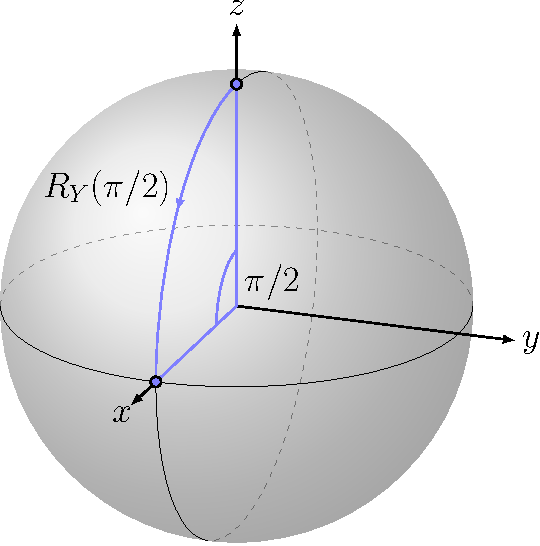
\includegraphics[width=0.5\textwidth]{lesson2/bloch_sphere_y_axis.pdf}

    \def\r{4}
    \tdplotsetmaincoords{70}{115}
    
    \begin{tikzpicture}[tdplot_main_coords,scale=0.7,every node/.style={scale=0.7}]

    \tdplotsetcoord{O}{0}{0}{0}

    \shade[tdplot_screen_coords,ball color=gray!40,opacity=0.5] (0,0,0) circle (\r);    % sphere
    \tdplotCsDrawLonCircle[tdplotCsFill/.style={blue!50,opacity=0.1},tdplotCsBack/.style={black!50,dashed},thin]{\r}{90}
    \tdplotCsDrawLatCircle[tdplotCsBack/.style={black!50,dashed}]{\r}{0}

    \draw[blue!50] (O) -- (\r,0,0);
    \draw[thick] (O) -- (0,\r,0);
    \draw[blue!50] (O) -- (0,0,\r);
    \draw[dashed,black!50] (O) -- (-\r,0,0);
    \draw[dashed,black!50] (O) -- (0,-\r,0);
    \draw[dashed,black!50] (O) -- (0,0,-\r);

    \tdplotsetthetaplanecoords{0}
    \draw[tdplot_rotated_coords,-,blue!50,very thick,decoration={markings, mark=at position 0.5 with {\arrow{latex}}},postaction={decorate}] (0:\r) arc (0:90:\r);
    \draw[tdplot_rotated_coords,-,blue!50] (0:0.3*\r) arc (0:90:0.3*\r);
    
    \tdplotCsDrawCircle[tdplotCsFill/.style=blue!50,thick]{\r}{0}{0}{88.5}
    \tdplotCsDrawCircle[tdplotCsFill/.style=blue!50,thick]{\r}{0}{90}{88.5}

    \draw[-latex,thick] (\r,0,0) -- (1.3*\r,0,0) node[pos=1.5] {\Large $x$};
    \draw[-latex,thick] (0,\r,0) -- (0,1.3*\r,0) node[pos=1.4] {\Large $y$};
    \draw[-latex,thick] (0,0,\r) -- (0,0,1.3*\r) node[pos=1.38] {\Large $z$};
    
    \node[] at (\r,0.5,-0.4) {\Large $|+\rangle$};
    \node[] at (0,0.35,\r+0.6) {\Large $|0\rangle$};

    \node[] at (\r,-0.5,3.5) {\Large $R_y(\pi/2)$};
    \end{tikzpicture}
    
    \caption[Rotation about $y$ axis.]{Rotation about the $Y$ axis by an angle $\pi/2$.}
    
    \label{fig:y-rot}
\end{figure}

Let's consider the example shown in Fig.~\ref{fig:y-rot}: we want to rotate around the y-axis through an angle of $\pi/2$, and our initial state is given by $\ket{0}$.  Let's start at the point $\ket{0}$, at the north pole of the sphere, and rotate around the y-axis. Going down along the surface by angle $\pi/2$, you see that we reach the state \ket{+}, which is an equal superposition of \ket{0} and \ket{1}.  For this $Y$ rotation, $\hat{n}$ simply becomes the unit vector along the positive y-axis, which we will just write $y$. Written out, we have
\begin{equation}
R_y(\pi / 2)\ket{0}=\ket{+}.
\end{equation}
(Be careful here; although this rotation took us from \ket{0} to \ket{+}, just like the Hadamard gate we have already seen, $H$ is not a $\pi/2$ $Y$ axis rotation.  Instead, $H$ is a $\pi$ rotation about the axis $(X+Z)/2$. See the exercises for more.)

\begin{figure}[H]
    \centering
    % 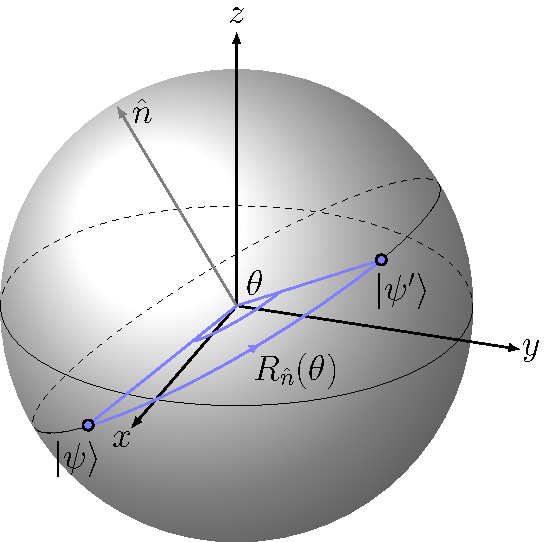
\includegraphics[width=0.5\textwidth]{lesson2/bloch_sphere_general_axis.pdf}

    \def\r{4}
    \def\alp{110}
    \def\bet{25}
    \def\eps{40}
    \tdplotsetmaincoords{70}{115}

    \begin{tikzpicture}[tdplot_main_coords,scale=0.7,every node/.style={scale=0.7}]

    \tdplotsetcoord{O}{0}{0}{0}
    \tdplotsetcoord{pointAxis}{\r}{\alp}{\bet}

    \shade[tdplot_screen_coords,ball color=gray!40,opacity=0.5] (0,0,0) circle (\r);    % sphere
    \tdplotCsDrawLatCircle[tdplotCsBack/.style={black!50,dashed}]{\r}{0}

    \pgfmathsetmacro\re {\r*cos(\eps)}
    \pgfmathsetmacro\ze {\r*sin(\eps)}
    \pgfmathsetmacro\coX{\ze*cos(\alp)*sin(\bet)}
    \pgfmathsetmacro\coY{\ze*sin(\alp)*sin(\bet)}
    \pgfmathsetmacro\coZ{\ze*cos(\bet)}
    \pgfmathsetmacro\length{sqrt(\coX*\coX+\coY*\coY+\coZ*\coZ)}
    \coordinate (pointAxis) at (\r*\coX/\length,\r*\coY/\length,\r*\coZ/\length);
    
    \draw[thick,-latex] (O) -- (pointAxis) node[anchor=east,yshift=4pt]{\Large $\hat{n}$};

    \draw[thick] (O) -- (\r,0,0);
    \draw[thick] (O) -- (0,\r,0);
    \draw[thick] (O) -- (0,0,\r);
    \draw[dashed,black!50] (O) -- (-\r,0,0);
    \draw[dashed,black!50] (O) -- (0,-\r,0);
    \draw[dashed,black!50] (O) -- (0,0,-\r);

    \draw[-latex,thick] (\r,0,0) -- (1.3*\r,0,0) node[pos=1.5] {\Large $x$};
    \draw[-latex,thick] (0,\r,0) -- (0,1.3*\r,0) node[pos=1.4] {\Large $y$};
    \draw[-latex,thick] (0,0,\r) -- (0,0,1.3*\r) node[pos=1.38] {\Large $z$};

    \tdplotCsDrawCircle[tdplotCsFill/.style={blue!50,opacity=0.1},tdplotCsBack/.style={black!50,dashed},thin]{\r}{\alp}{\bet}{\eps}

    \tdplotsetrotatedcoords{\alp}{\bet}{0}
    \coordinate (coffs) at (\coX,\coY,\coZ);
    \tdplotsetrotatedcoordsorigin{(coffs)}
    
    \draw[tdplot_rotated_coords,blue!50,very thick,decoration={markings, mark=at position 0.6 with {\arrow{latex}}},postaction={decorate}] (-160:\re) arc (-160:-30:\re) node[pos=0.6,below,black,yshift=-4pt] {\Large $R_{\hat{n}}(\theta)$};
    
    \draw[tdplot_rotated_coords,blue!50] (-160:0.3*\re) arc (-160:-30:0.3*\re);
    \draw[tdplot_rotated_coords,blue!50] (0,0,0) -- (-160:\re) node[black,anchor=east,xshift=-1pt,yshift=-4pt]{\Large $|\psi\rangle$};
    \draw[tdplot_rotated_coords,blue!50] (0,0,0) -- (-30:\re) node[anchor=north,black,yshift=-3pt]{\Large $|\psi'\rangle$};

    \tdplotCsDrawCircle[tdplotCsFill/.style=blue!50,thick]{\r}{-34}{27.9}{88.5}
    \tdplotCsDrawCircle[tdplotCsFill/.style=blue!50,thick]{\r}{85.5}{72.3}{88.5}
    \end{tikzpicture}
    
    \caption{Rotation about an arbitrary axis $\hat{n}$.}
    
    \label{fig:arb-rot}
\end{figure}

More generally, it is not necessary to rotate about one of these orthogonal axes; you can rotate about any axis that you want, as in Fig.~\ref{fig:arb-rot}. You are rotating in the plane defined by your chosen axis and parameterized by the angle $\theta$. Take some initial state $\ket{\psi}$ that's on the surface of the Bloch sphere, follow the surface and end at some new state $\ket{\psi'}$.  (Note that the plane a particular state is rotating in does not have to pass through the center of the Bloch sphere, but the axis of rotation is normal to the plane.) 

So you can see that you can work in the matrix representation or you can work also in the Bloch sphere representation for single-qubit operations.


% $U_{00}$, $U_{01}$, $U_{10}$, $U_{11}$ 

\section{Measurement}
\label{sec:measurement}

Now, let's consider measurements and how they can extract information from qubits~\footnote{The type of measurements we consider in this book are \emph{projective measurements}, as discussed more in the next chapter. There are other types of measurement that you will learn about in advanced quantum classes.}. Basically a measurement asks the question: is my qubit in the state $\ket{0}$ or is it in the state $\ket{1}$? You can think of a measurement as a big box and you feed it your prepared state, as shown in Fig.~\ref{fig:z-measure}. Here, we consider a general state given by $\ket{\psi} = \alpha\ket{0}+\beta\ket{1}$, and the measurement operation tells you which state it is in. Usually there are only two possible values that can come out of a measurement device, which we will assign the values $+1$ and $-1$.

\begin{figure}[H]
    \centering
    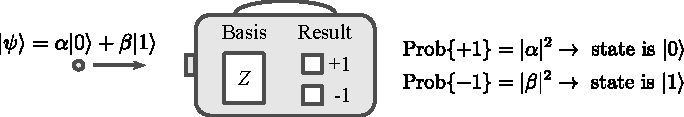
\includegraphics[width=0.8\textwidth]{lesson2/2-2_measurement_Z.pdf}
    \caption{Measurement in the $Z$ basis.}
    \label{fig:z-measure}
\end{figure}

The probabilities of these measurement outcomes, corresponding to state \ket{0} and state \ket{1}, are given by their probability amplitudes. The probability of getting a $+1$ outcome is given by $|\alpha|^2$ and the probability of a $-1$ outcome is given by $|\beta|^2$. Immediately after the measurement, the state \textbf{\emph{collapses}}\index{state collapse} either onto \ket{0} or onto \ket{1}, so if you get a $+1$ outcome you can be sure that immediately after the measurement the state is in the state \ket{0}, or if you get a $-1$ then the state of the system has changed from the initial $\ket{\psi}$ and is \ket{1},
\begin{align}
\operatorname{Prob}\{+1\}=|\alpha|^2 \rightarrow \textrm{state is } |0\rangle \\
\operatorname{Prob}\{-1\}=|\beta|^2 \rightarrow \textrm{state is } |1\rangle.
\end{align}

(Mathematically speaking, the $\pm 1$ outcomes of the measurement are the \emph{eigenvalues} corresponding to the \textbf{\emph{eigenvectors}}\index{eigenvector} of the Pauli $Z$ operator.  One way to remember which value corresponds to which vector is that $+1$ corresponds to \ket{0}, and $(-1)^0 = +1$, while $-1$ corresponds to \ket{1}, and $(-1)^1 = -1$.)

We refer to this particular measurement as a measurement in the \textbf{\emph{computational basis}\index{computational basis}} or in the Pauli $Z$ basis. This already hints at the fact that this is not the only measurement we can do. We can also ask the following question: is the state in the $\ket{+}$ state or in the $\ket{-}$ state? We can answer this question by rewriting our original state
\begin{equation}
    \psi\rangle=\alpha|0\rangle+\beta|1\rangle
    \label{eq:superposition_basisZ}
\end{equation}
using the algebraic identities
\begin{equation}
|0\rangle=\frac{1}{\sqrt{2}}(|+\rangle+|-\rangle) \quad|1\rangle=\frac{1}{\sqrt{2}}(|+\rangle-|-\rangle).
\end{equation}
Notice that $\ket{0}$ is given by an equal superposition of the $\ket{+}$ state with the $\ket{-}$ state and the state $\ket{1}$ is also an equal superposition of $\ket{+}$ and $\ket{-}$, but this time with a minus phase in front of the $\ket{-}$ state. We can rewrite our original state $\ket{\psi}$ in terms of these \ket{+} and \ket{-} states, but this time the probability amplitudes are
%for the state plus is $\alpha+\beta$ renormalized by the square root of two, and the probability amplitude for the minus state is $\alpha-\beta$,
\begin{equation}
    \ket{\psi}=\frac{\alpha+\beta}{\sqrt{2}}\ket{+}+\frac{\alpha-\beta}{\sqrt{2}}\ket{-}.
    \label{eq:superposition_basisX}
\end{equation}
Again, we can feed our qubit into the measurement device and it will give us an answer $\ket{+}$ or $\ket{-}$ with the following probabilities,
\begin{align}
\label{eq:plus-measurement}
\operatorname{Prob}\{+1\}=\frac{|\alpha+\beta|^2}{2} \rightarrow \textrm{state is } |+\rangle \\
\label{eq:minus-measurement}
\operatorname{Prob}\{-1\}=\frac{|\alpha-\beta|^2}{2} \rightarrow \textrm{state is } |-\rangle.
\end{align}
You can see that the probabilities still depend on $\alpha$ and $\beta$, but they're not just $|\alpha|^2$ and $|\beta|^2$.
%they're in fact alpha plus beta the whole thing mod squared and alpha minus beta the whole thing squared and both of them are divided by two. 
Because we were asking a different question (whether the state state is in $\ket{+}$ or $\ket{-}$), the state changes from $\ket{\psi}$ and goes to $\ket{+}$ or $\ket{-}$ after the measurement, depending on the measurement outcome. This measurement is known as measurement in the Pauli $X$ basis, and is shown in Fig.~\ref{fig:x-meas}.

\begin{figure}[H]
    \centering
    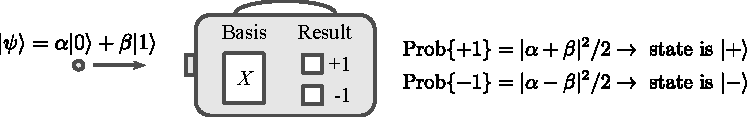
\includegraphics[width=0.85\textwidth]{lesson2/2-2_measurement_X.pdf}
    \caption{Measurement in the Pauli $X$ basis.}
    \label{fig:x-meas}
\end{figure}

In fact, you can measure in any basis that you can think of.  This is explored more in the exercises.

We have been using this word \textbf{\emph{basis}}\index{basis}, but what is a ``basis''? Maybe you remember from your linear algebra class that a basis is a set of vectors that allows you to write down any vector that you can think of. If we have a general vector $\ket{\psi}$, we can express it in terms of the basis states $\ket{0}$ and \ket{1}, as shown in Eq.~(\ref{eq:superposition_basisZ}).
But the same state $|\psi\rangle$ can be expressed in terms of the states $|\pm\rangle$, as we have seen in Eq.~(\ref{eq:superposition_basisX}).
We do not have to use only the Pauli $Z$ or the Pauli $X$ bases, however.
Let's say you want to write the state $|\psi\rangle$ in terms of the states $\ket{i}$ and $\ket{-i}$.
This is known as the Pauli $Y$ basis, and their vector representations are given as
\begin{align}
    |i\rangle=\frac{1}{\sqrt{2}}\left(\begin{array}{l}1 \\ i\end{array}\right) \quad|-i\rangle=\frac{1}{\sqrt{2}}\left(\begin{array}{c}1 \\ -i\end{array}\right).
    \label{eq:Pauli_Y_basis}
\end{align}
%So it's just (1, i) and (1, -i) with the appropriate normalization factor in front, and 
Then the state $|\psi\rangle$ can be rewritten as
\begin{equation}
    |\psi\rangle=\frac{\alpha-i \beta}{\sqrt{2}}|i\rangle+\frac{\alpha+i \beta}{\sqrt{2}}|-i\rangle.
    \label{eq:superposition_basisY}
\end{equation}
The expressions in Eqs.~(\ref{eq:superposition_basisZ}), (\ref{eq:superposition_basisX}), and (\ref{eq:superposition_basisY}) look very different but they represent the same state: the state has not changed.
It's just that our description of the state is a different because we have chosen a different basis to express it.

Another important concept is the \textbf{\emph{inner product}}\index{inner product}. The inner product is basically a dot product between two vectors.
It tells us the ``overlap'' between two quantum states, which is a measure of how similar the states are. To write down the inner product in the notation we use in this book, first we have to define a \textbf{\emph{bra}}\index{bra}. Given a state $\ket{\psi}$, the corresponding bra is its adjoint. The bra of state $\ket{\psi}$ is given as the dagger of the original column vector,
\begin{equation}
\langle\psi|=(|\psi\rangle)^{\dagger}=\left(\begin{array}{l}
\alpha \\
\beta
\end{array}\right)^{\dagger}=\left(\begin{array}{ll}
\alpha^{*} & \beta^{*}
\end{array}\right).
\end{equation}
We applied the same trick we used for defining the adjoint of unitary operations: take the complex conjugate of $\alpha$ and $\beta$ and then transpose the column vector, which turns it into a row vector. Now we can find the inner product between two arbitrary states, $\ket{\psi} = \alpha\ket{0} + \beta\ket{1}$ and $\ket{\phi} = \gamma\ket{0} + \delta\ket{1}$. We write it as 
\begin{equation}
\langle\phi \mid \psi\rangle=\left(\begin{array}{ll}
\gamma^{*} & \delta^{*}
\end{array}\right)\left(\begin{array}{c}
\alpha \\
\beta
\end{array}\right)=\alpha \gamma^{*}+\beta \delta^{*}.
\end{equation}
This should be no surprise if you remember your dot products from your linear linear algebra class.
Unlike the dot product from your linear algebra class, the inner product can be a complex number.
This means that in general $\langle\psi|\phi\rangle \neq \langle\phi|\psi\rangle$.

Also notice that if we take the inner product of the state with itself, we get this expression:
\begin{equation}
\langle\psi \mid \psi\rangle=|\alpha|^{2}+|\beta|^{2}=1.
\end{equation}
Mod alpha squared plus mod beta squared will be equal to one, if the state is properly normalized.

For two different states, we can also come across the scenario where the inner product between two states is zero,
\begin{equation}
\langle\phi \mid \psi\rangle=0.
\end{equation}
In that case, we say that the two states are \textbf{\emph{orthogonal}}.

Being equipped with the knowledge of the inner product, we can address the following question: how can we compute the probabilities of different outcomes when measuring the state in a particular basis?
Given our general state $\ket{\psi}$, let's say that we want to measure in some arbitrary basis given by the states $\ket{b_{+1}}$ and $\ket{b_{-1}}$.
State $\ket{b_{+1}}$ represents the +1 outcome of the measurement, while the state $\ket{b_{-1}}$ represents the -1 outcome of the measurement.
We are asking the question: is my state $|\psi\rangle$ in the state $|b_{+1}\rangle$ or is my state in the state $|b_{-1}\rangle$?
To answer this, we take the inner product between $\ket{b_{+1}}$ and $\ket{\psi}$, take the modulus and we square it, and that gives us the probability of a $+1$ outcome. Correspondingly, the probability of the $-1$ outcome is given by the inner product between $\ket{b_{-1}}$ and $\ket{\psi}$ modulus squared,
\begin{equation}
\begin{aligned}
    \operatorname{Prob}\{+1\}&=\left|\left\langle b_{0}\mid \psi\right\rangle\right|^{2}, \\
    \operatorname{Prob}\{-1\}&=\left|\left\langle b_{1}\mid \psi\right\rangle\right|^{2}.
\end{aligned}
\end{equation}

Let's illustrate this with a familiar example. We start by measuring in the Pauli Z basis. This means that our basis states are $|b_{+1}\rangle=|0\rangle$, and $|b_{-1}\rangle=|1\rangle$. The probabilities of the two outcomes are then given by
\begin{equation}
\begin{aligned}
    \operatorname{Prob}\{+1\} &=|\langle 0 \mid \psi\rangle|^2=|\alpha|^2, \\
    \operatorname{Prob}\{-1\} &=|\langle 1 \mid \psi\rangle|^2=|\beta|^2.
\end{aligned}
\end{equation}

We can now apply this procedure to a new scenario. Let's measure our state $|\psi\rangle$ in the Pauli $Y$ basis.
Our basis states are given by $|b_{+1}\rangle=|i\rangle$, and $|b_{-1}\rangle=|-i\rangle$.
Using the definition of the Pauli $Y$ basis states in Eq.~(\ref{eq:Pauli_Y_basis}), we can compute the probabilities as follows,
\begin{equation}
\begin{aligned}
    \operatorname{Prob}\{+1\} &=|\langle i \mid \psi\rangle|^2=\frac{|\alpha-i \beta|^2}{2}, \\
    \operatorname{Prob}\{-1\} &=|\langle-i \mid \psi\rangle|^2=\frac{|\alpha+i \beta|^2}{2}.
\end{aligned}
\end{equation}
Notice that the for the case of measuring in the Pauli $Y$ basis, the inner product is a complex number, but the probability obtained from the inner product is a real number, as one would expect.

% To summarize the measurement process, start with some initial state written in some basis,
% and then say, okay I want to perform a measurement in a given basis described by these basis states $\ket{b_0}$ and $\ket{b_1}$. If my outcome is $+1$, which happens with the probability given by the inner product between the basis state with the original state modulus squared, then my post measurement state is given by $\ket{b_0}$. Or, if I get the $-1$ outcome, which happens with probability given by the inner product of $\ket{b_1}$ with the initial state $\ket{\psi}$ modulus squared, then my post measurement state is given by $\ket{b_1}$.

There is something very important to keep in mind: the measurement outcome is only $+1$ or $-1$. A single measurement does not reveal any information about the probability amplitudes $\alpha$ and $\beta$.
In the next section, we will consider multiple measurements, which can be used to obtain information about the probabilities of measurement outcomes.



\section{Probabilities, expectation, variance}

We have seen how the measurement process can be described mathematically, and how the inner product is used to compute the probabilities of various measurement outcomes.
In this section, we will see how we can also compute the expectation value of a measurement outcomes as well its variance.
Up to this point, we have only measured the qubit once, as in Figs.~\ref{fig:z-measure} and \ref{fig:x-meas}.
This is known as \textbf{\emph{single-shot measurement}}\index{single-shot measurement}.
Now let's consider the scenario where we have many copies of the same state \ket{\psi} and we keep measuring them again and again by feeding them to our measurement device, as shown in Fig.~\ref{fig:many-copies}. What comes out of the measurement device is a string of $+1$ and $-1$ results.
\begin{figure}[H]
    \centering
    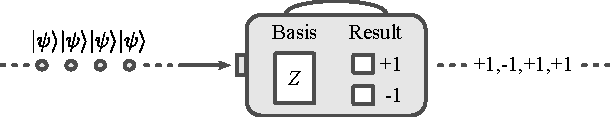
\includegraphics[width=0.75\textwidth]{lesson2/2-2_measurement_many.pdf}
    \caption[Repeated measurements.]{Repeated measurements of many copies of the state $|\psi\rangle$.}
    \label{fig:many-copies}
\end{figure}

We can count the number of $+1$ outcomes, which we denote by $N(+1)$, and we can count the number of $-1$ outcomes, which we denote by $N(-1)$. Intuitively, the ratio between the number of $+1$ outcomes to the total number of measurements will be approximately equal to the probability of obtaining the plus one outcome, which is $|\alpha|^2$, and similarly for the fraction of the number of $-1$ outcomes, which will be very close to $|\beta|^2$,
\begin{equation}
    \frac{N(+1)}{N(+1)+N(-1)} \approx|\alpha|^{2}, \qquad \frac{N(-1)}{N(+1)+N(-1)} \approx|\beta|^{2}.
\end{equation}
The approximation becomes more accurate as we increase the number of times the measurement is repeated.

In order to extract information about the probabilities of measurement outcomes, we have to repeat the same measurement on a fresh copy $|\psi\rangle$. Because these measurements are random, we're not going to get the same answer every time. However, we can ask the question: what is the expected result when we measure in the Pauli $Z$ basis? Maybe you remember from your probability course that the \textbf{\emph{expectation value}}\index{expectation value} of some random variable is the sum of the probability of each possible outcome times its value. Let's call our variable $Z$ because we are measuring in the Pauli $Z$ basis.  Its expectation value is given by the probability of the $+1$ outcome times $+1$ (the value of the outcome), plus the probability of $-1$ times the value of the outcome, which is in this case $-1$.  The probability of $+1$ remains $|\alpha|^2$, and the probability of the $-1$ outcome is given by $|\beta|^2$, but this time we are multiplying it by $-1$. So the expectation value when we measure in the Pauli Z basis is given by the expression
\begin{equation}
\begin{aligned}
    \mathbb{E}[Z] &=\operatorname{Prob}{+1} \cdot(+1)+\operatorname{Prob}{-1} \cdot(-1) \\
    &=|\alpha|^{2}-|\beta|^{2}.
    \label{eq:expectation_Z}
\end{aligned}
\end{equation}

In Dirac notation, we write it as follows. We write the operator in which basis we are measuring, for example the Pauli $Z$, and we enclose it in the angle brackets. This is a shorthand for saying that we are multiplying the bra of state $\bra{\psi}$ times the $Z$ operator times the ket of state $\ket{\psi}$,

\begin{equation}
    \langle Z\rangle=\langle\psi|Z| \psi\rangle.
\end{equation}

Let's check that this produces the expected result. Take the Pauli $Z$ operator and sandwich it between the bra $\langle\psi|$ and the ket $|\psi\rangle$. When we multiply this out, we get the following expression,
\begin{equation}
    \begin{aligned}
    \langle Z\rangle &=\left(\begin{array}{ll}
    \alpha^{*} & \beta^{*}
    \end{array}\right)\left(\begin{array}{cc}
    1 & 0 \\
    0 & -1
    \end{array}\right)\left(\begin{array}{l}
    \alpha \\
    \beta
    \end{array}\right) \\
    &=\left(\begin{array}{ll}
    \alpha^{*} & \beta^{*}
    \end{array}\right)\left(\begin{array}{c}
    \alpha \\
    -\beta
    \end{array}\right) \\
    &=|\alpha|^{2}-|\beta|^{2}.
    \end{aligned}
    \label{eq:z-expectation}
\end{equation}
This agrees with our expression from Eq.~(\ref{eq:expectation_Z}).

Because the outputs of the measurements are random we expect some degree of variance. The variance of a classical random variable $A$ is given by the expectation value of the square of that variable minus the square of the expectation value of that variable,
\begin{equation}
    \operatorname{Var}[A] =\mathbb{E}\left[A^{2}\right]-\mathbb{E}[A]^{2}.
\end{equation}
We can compute the variance of the Pauli $Z$ operator.
We have already computed the expectation value of $Z$ in Eq.~\ref{eq:z-expectation}. We therefore have to compute the expectation value of $Z^2$. That's the probability of getting a $+1$ outcome times $(+1)^2$ which is just $+1$.  The probability of the $-1$ outcome times $(-1)^2$, which is $1$, so actually what we get is
\begin{equation}
\begin{aligned}
    \mathbb{E}\left[Z^{2}\right] &=\operatorname{Prob}\{+1\} \cdot(+1)^{2}+\operatorname{Prob}\{-1\} \cdot(-1)^{2} \\
    &=|\alpha|^{2}+|\beta|^{2}.
\end{aligned}
\end{equation}
If the state is properly normalized, and it should be, then $\mathbb{E}[Z^{2}]=1$.
In fact, we could have guessed this without the explicit calculation by realizing that $Z^2=I$.
So that variance of the Pauli $Z$ operator can be written as
\begin{equation}
    \operatorname{Var}[Z] = 1 - \langle Z \rangle^2.
\end{equation}

Often in physics you will see that the variance is referred to as \textbf{\emph{fluctuations}}\index{fluctuations}, denoted by $(\Delta Z)^2$. In the Dirac notation, we again have this expression,
\begin{equation}
    (\Delta Z)^{2} \equiv \operatorname{Var}[Z] = \left\langle Z^{2}\right\rangle-\langle Z\rangle^{2}.
\end{equation}





\section{Multiple Qubits}
\label{sec:multi-qubit}

Now, let's consider how to write down the quantum state of multiple qubits. Let's start with the very simple task of writing down the state of two qubits. If we have two classical bits, they can be in four different states: $00$, $01$, $10$, or $11$. So what's the case for quantum bits? We need to switch to the Dirac notation, and we still have four possible states: $\ket{00}$, $\ket{01}$, $\ket{10}$, and $\ket{11}$. Any general state of two qubits can be written as a superposition of these four states weighted by their respective probability amplitudes $\alpha$, $\beta$, $\gamma$ and $\delta$, 
\begin{equation}
    |\psi\rangle=\alpha|00\rangle+\beta|01\rangle+\gamma|10\rangle+\delta|11\rangle.
    \label{eq:superposition_2qubits}
\end{equation}
The state $|\psi\rangle$ must be normalized, just like in the case of single-qubit states. The normalization condition is as follows,
\begin{equation}
    |\alpha|^2+|\beta|^2+|\gamma|^2+|\delta|^2 = 1,
\end{equation}
the moduli of all the probability amplitudes squared must sum it up to one.
In vector notation, we can write these kets as follows,
\begin{equation}
|00\rangle=\left(\begin{array}{l}
1 \\
0 \\
0 \\
0
\end{array}\right), \quad |01\rangle=\left(\begin{array}{l}
0 \\
1 \\
0 \\
0
\end{array}\right), \quad |10\rangle=\left(\begin{array}{l}
0 \\
0 \\
1 \\
0
\end{array}\right), \quad |11\rangle=\left(\begin{array}{l}
0 \\
0 \\
0 \\
1
\end{array}\right).
\end{equation}
We can easily check that these states are orthogonal to each other, and that they form a basis for the space of two-qubit states.
We can rewrite our general two-qubit superposition in Eq.~(\ref{eq:superposition_2qubits}) in the vector form as follows,
\begin{equation}
\ket{\psi}=\alpha\left(\begin{array}{l}
1 \\
0 \\
0 \\
0
\end{array}\right) + \beta\left(\begin{array}{l}
0 \\
1 \\
0 \\
0
\end{array}\right)+\gamma\left(\begin{array}{l}
0 \\
0 \\
1 \\
0
\end{array}\right)+\delta\left(\begin{array}{l}
0 \\
0 \\
0 \\
1
\end{array}\right)=\left(\begin{array}{l}
\alpha \\
\beta \\
\gamma \\
\delta
\end{array}\right).
\end{equation}

The mathematical concept behind being able to write the basis states in this fashion is the \textbf{\emph{tensor product}}\index{tensor product}~\footnote{There are actually multiple types of tensor products; by one definition, a tensor is like an $n$-dimensional matrix instead of the customary two-dimensional one.  In this book, we will use tensors in a fashion that expands the vector or matrix size, instead of making it into a multidimensional object.}.
The tensor product allows us to construct the vector representation of two qubits, given the states of the individual qubits.
Let's say that the first qubit is in the state $|a\rangle=(a_1,a_2)^T$, while the second qubit is in a different state $|b\rangle=(b_1,b_2)^T$.
The two-qubit state can then be expressed as
\begin{equation}
|a\rangle \otimes|b\rangle=\left(\begin{array}{l}
a_{1} \\
a_{2}
\end{array}\right) \otimes\left(\begin{array}{l}
b_{1} \\
b_{2}
\end{array}\right) \equiv\left(\begin{array}{l}
a_{1}\left(\begin{array}{l}
b_{1} \\
b_{2}
\end{array}\right) \\
a_{2}\left(\begin{array}{l}
b_{1} \\
b_{2}
\end{array}\right)
\end{array}\right)=\left(\begin{array}{l}
a_{1} b_{1} \\
a_{1} b_{2} \\
a_{2} b_{1} \\
a_{2} b_{2}
\end{array}\right),
\label{eq:tensor_product_state}
\end{equation}
where the symbol $\otimes$ denotes the tensor product.

To calculate the product, take the first probability amplitude $a_1$ times the whole column vector for $\ket{b}$. That will give us the first two elements in our new four dimensional vector.  $a_1$ times $b_1$ goes into the first entry in the resulting vector, $a_1$ times $b_2$ goes in the second entry. The bottom two elements are given by $a_2$ multiplying the whole column vector of $\ket{b}$, giving us $a_2$ times $b_1$ and $a_2$ times $b_2$.
Note that the tensor product symbol is often omitted to save space, and two-qubit state is written in a number of equivalent ways,
\begin{equation}
    |a\rangle\otimes|b\rangle = |a\rangle|b\rangle = |a,b\rangle = |ab\rangle.
\end{equation}

For example, if we have two qubits and the first qubit is in the state $\ket{0}$, and the second qubit is in the state $|1\rangle$, we write the two-qubit state as
\begin{equation}
|0\rangle \otimes|1\rangle=\left(\begin{array}{l}
1 \\
0
\end{array}\right) \otimes\left(\begin{array}{l}
0 \\
1
\end{array}\right)=\left(\begin{array}{l}
0 \\
1 \\
0 \\
0
\end{array}\right).
\end{equation}
We can the same logic to more complicated states. Let's say we have the tensor product of $\ket{1}$ with $\ket{-}$,
\begin{equation}
|1\rangle \otimes|-\rangle=\left(\begin{array}{l}
0 \\
1
\end{array}\right) \otimes \frac{1}{\sqrt{2}}\left(\begin{array}{c}
1 \\
-1
\end{array}\right)=\frac{1}{\sqrt{2}}\left(\begin{array}{c}
0 \\
0 \\
1 \\
-1
\end{array}\right).
\end{equation}

The tensor product is very general and goes beyond the case of two qubits. Given two vectors with $m$ and $n$ entries, their tensor product will be a vector with $mn$ entries in it. When dealing with qubits, our vectors will generally have a length that is a power of two since each qubit added to the system doubles the number of entries in the vector when we take the tensor product.

Notice that if the individual quantum states are normalized, their tensor product is automatically normalized as well.
And finally, be careful: just as with ordinary matrix products, the order of vectors (kets) written in a tensor product matters. This will be explored in detail in the exercises.

Having seen how we can describe multi-qubit states, it is time to learn how we can write down the operations that act on such states.
The logic is identical to our previous discussion and relies on the use of tensor products.
Consider operator $A$ acting on the first qubit, and operator $B$ acting on the second qubit.
The two-qubit operator is then described by the tensor product of the two operators,
\begin{equation}
\begin{aligned}
A \otimes B &=\left(\begin{array}{ll}
A_{11} & A_{12} \\
A_{21} & A_{22}
\end{array}\right) \otimes\left(\begin{array}{ll}
B_{11} & B_{12} \\
B_{21} & B_{22}
\end{array}\right) \\
&=\left(\begin{array}{lll}
A_{11}\left(\begin{array}{ll}
B_{11} & B_{12} \\
B_{21} & B_{22}
\end{array}\right) & A_{12}\left(\begin{array}{ll}
B_{11} & B_{12} \\
B_{21} & B_{22}
\end{array}\right) \\
A_{21}\left(\begin{array}{ll}
B_{11} & B_{12} \\
B_{21} & B_{22}
\end{array}\right) & A_{22}\left(\begin{array}{ll}
B_{11} & B_{12} \\
B_{21} & B_{22}
\end{array}\right)
\end{array}\right) \\
&=\left(\begin{array}{llll}
A_{11} B_{11} & A_{11} B_{12} & A_{12} B_{11} & A_{12} B_{12} \\
A_{11} B_{21} & A_{11} B_{22} & A_{12} B_{21} & A_{12} B_{22} \\
A_{21} B_{11} & A_{21} B_{12} & A_{22} B_{11} & A_{22} B_{12} \\
A_{21} B_{21} & A_{21} B_{22} & A_{22} B_{21} & A_{22} B_{22}
\end{array}\right)
\end{aligned}
\end{equation}
In the upper left, we have $A_{11}$ times the matrix representation of $B$. In the upper right square, we have the element $A_{12}$ times the whole matrix $B$. In the lower left, we have  $A_{21}$ times matrix $B$, and finally in the lower right $A_{22}$ times matrix $B$.

Having to multiply the individual matrix representations of the operators is quite cumbersome.
It is often more convenient to work in the Dirac notation to find out the action of the multi-qubit operator on the state.
Let's apply the two-qubit operator $A\otimes B$ to the two-qubit state $|a\rangle\otimes|b\rangle$ in Eq.~(\ref{eq:tensor_product_state}),
\begin{equation}
    (A\otimes B) |a\rangle\otimes|b\rangle = (A|a\rangle) \otimes (B|b\rangle).
\end{equation}
We can first compute the effect $A$ on $|a\rangle$, and of $B$ on $|b\rangle$ individually, and then take the tensor product.

As an example, consider applying a Pauli $X$ to the first qubit of the state $|\psi\rangle$ in Eq.~(\ref{eq:superposition_2qubits}), while leaving the second qubit alone. Leaving a qubit alone just means that we apply the identity operator to it. This is written as
\begin{equation}
\begin{aligned}
    (X \otimes I)|\psi\rangle &=X \otimes I(\alpha|00\rangle+\beta|01\rangle+\gamma|10\rangle+\delta|11\rangle) \\
    &=\alpha|10\rangle+\beta|11\rangle+\gamma|00\rangle+\delta|01\rangle
\end{aligned}
\end{equation}
If we write out the tensor of the operators, we have
\begin{equation}
X \otimes I=\left(\begin{array}{ll}
0 & 1 \\
1 & 0
\end{array}\right) \otimes\left(\begin{array}{ll}
1 & 0 \\
0 & 1
\end{array}\right)=\left(\begin{array}{llll}
0 & 0 & 1 & 0 \\
0 & 0 & 0 & 1 \\
1 & 0 & 0 & 0 \\
0 & 1 & 0 & 0
\end{array}\right).
\end{equation}

Note that, unlike ordinary matrix multiplication, two matrices being tensored do not have to have a dimension in common. They can be any size. If $A$ is an $l\times m$ matrix and $B$ is an $n \times p$ matrix, the result will be an $ln \times mp$ matrix.

Similarly to tensor product of two kets, where we often drop the twensor product symbol, we can do something the same with tensoring operators.
Though we have to be careful to keep in mind that doing ordinary matrix multiplication.
A good strategy is to add indices to the operators as a reminder that they act on different qubits,
\begin{equation}
    A \otimes B \equiv A_1B_2.
\end{equation}

Finally, by now you have probably recognized that one of the great advantages of the Dirac notation is its compactness. Two qubits can have four possible states, three qubits can have eight possible states, and so on; for $n$ qubits, the state vector is $2^n$ elements long when written out. But most of the time, we don't need to write out the entire state.  You have seen that the individual basis states are more compactly written, such as writing $\ket{00}$ instead of the whole four-element vector, let alone writing out the whole sixteen elements of the four-qubit state $\ket{0000}$. But more generally, even when dealing with an arbitrary state $\ket{\psi}$, we only need to write out the \textbf{\emph{nonzero}} elements, allowing us to ignore the zero elements.  Thus, a four-qubit superposition of the all-zeroes and all-ones states only requires us to write $\ket{\psi} = (\ket{0000} + \ket{1111})/\sqrt{2}$, saving our hands, our pens, and ultimately being easier cognitively as well~\footnote{If you are familiar with the execution of matrix math in high-performance computing, the Dirac and tensor notations are equivalent to a \emph{sparse representation}, keeping a list of nonzero elements instead of all of them.}.

\if0
$\left(\begin{array}{ll}
1 & 0 \\
0 & 1
\end{array}\right)$

$\left(\begin{array}{ll}
0 & 1 \\
1 & 0
\end{array}\right)$
\fi

\newpage
\begin{exercises}
\exer{Consider the following quantum state:}
\begin{equation*}
\ket{\psi} = \frac{\sqrt{3}}{2}\ket{0} + \frac{1}{2}\ket{1}
\end{equation*}
\subexer{Find the probability of measuring a zero.}
\subexer{Find the probability of measuring a one.}
\exer{Write out the vectors corresponding to the following tensor products. Confirm that the vectors remain normalized. Note that the order of writing the qubits matters, but the order of taking the products does not.} \subexer{$\ket{+}\otimes \ket{1}$.}
\subexer{$\ket{1}\otimes \ket{+}$.}
\subexer{$\ket{+}\otimes \ket{+}$.}
\subexer{$\ket{-}\otimes \ket{+}$.}
\subexer{$\ket{+}\otimes \ket{-}$.}
\subexer{$\ket{-}\otimes \ket{-}$.}
\subexer{$\ket{0}\otimes \ket{0} \otimes\ket{0}$.}
\subexer{$\ket{0}\otimes \ket{0} \otimes\ket{1}$.}
\subexer{$\ket{0}\otimes \ket{1} \otimes\ket{0}$.}
\subexer{$\ket{1}\otimes \ket{0} \otimes\ket{0}$.}
\subexer{$\ket{1}\otimes \ket{1} \otimes\ket{1}$.}
\subexer{$\ket{1}\otimes \ket{+} \otimes\ket{0}$.}

\exer{Write out the matrices corresponding to the following tensor products.} \subexer{$X\otimes X$.}
\subexer{$Z\otimes Z$.}
\subexer{$I\otimes X$.}
\subexer{$I\otimes Z$.}
\subexer{$X\otimes Z$.}
\subexer{$Z\otimes X$.}

\exer{Find the expectation value $\langle Z\rangle$ for the following single-qubit states.}
\subexer{$\ket{0}$}
\subexer{$\ket{1}$}
\subexer{$\ket{+}$}
\subexer{$\ket{-}$}
\subexer{$\frac{\sqrt{3}}{2}\ket{0} + \frac{1}{2}\ket{1}$}

\exer{Since we can find the expectation value of $Z$, you might suspect that we can do the same for $X$. Find the expectation value $\langle X\rangle$ for the following single-qubit states.}
\subexer{$\ket{0}$}
\subexer{$\ket{1}$}
\subexer{$\ket{+}$}
\subexer{$\ket{-}$}
\subexer{$\frac{\sqrt{3}}{2}\ket{0} + \frac{1}{2}\ket{1}$}

\exer{We said above that the Hadamard gate is not just a y-axis rotation.  To explore this further, calculate the following. \\
Use $\ket{\lambda_{+}} = \frac{\sqrt{2 + \sqrt{2}}}{2}\ket{0}+\frac{1}{\sqrt{2(2 + \sqrt{2})}}\ket{1}$ and $\ket{\lambda_{-}}=\frac{\sqrt{2 - \sqrt{2}}}{2}\ket{0} - \frac{1}{\sqrt{2(2 - \sqrt{2})}}\ket{1}$.
\subexer{$H\ket{i}$}
\subexer{$R_Y(\pi/2)\ket{i}$}
\subexer{$R_Y(\pi)\ket{i}$}
\subexer{$H(\sqrt{3}\ket{0}+\ket{1})/\sqrt{2}$}
\subexer{$R_Y(\pi/2)(\sqrt{3}\ket{0}+\ket{1})/\sqrt{2}$}
\subexer{$R_Y(\pi)(\sqrt{3}\ket{0}+\ket{1})/\sqrt{2}$}
\subexer{$H\ket{\lambda_+}$}
\subexer{$H\ket{\lambda_-}$}
\subexer{$R_Y(\pi/2)\ket{\lambda_+}$}
\subexer{$R_Y(\pi/2)\ket{\lambda_-}$}
\subexer{$R_Y(\pi)\ket{\lambda_+}$}
\subexer{$R_Y(\pi)\ket{\lambda_-}$}
}
% \exer{
% \label{ex:dirac-notation-measurement}
% Let's explore single-qubit measurement in more depth. This will come in handy when we explore entanglement swapping in Sec.~\ref{sec:12-3_reaching_for_distance}. Another way of expressing measurement is to use $\operatorname{Prob}(i) = \bra{\psi}M_i\ket{\psi}$, where $\{M_i\}$ corresponds to the set of outcomes of our measurement operation. Each $M_i$ is written as an operator, $M_i = \ketbra{\psi_i}{\psi_i}$, and assuming there are two outcomes to the operation, $\pm 1$, then we have $M_{+1} = \ketbra{0}{0}$ and $M_{-1} = \ketbra{1}{1}$. Sometimes, we will write $M_{+1}^Z$ or $\Pi_{+1}^Z$ for measurement in the $Z$ basis, or even just $Z$.
% \subexer{
% Show that $\bra{\psi}M_i\ket{\psi}$ gives $|\alpha|^2$ and $|\beta|^2$ for \ket{0} and \ket{1}.
% }
% \subexer{
% Find the set of operators $\{M_i\}$ when measuring in the $X$ basis. Show that they produce the same probabilities as Eq.~\ref{eq:plus-measurement} and \ref{eq:minus-measurement}.
% }
% \subexer{One way to find the post-measurement state of a state is
% $$\ket{\psi'} = \frac{M_i\ket{\psi}}{\sqrt{\bra{\psi} M_i\ket{\psi}}}$$ when the outcome is $i$. Show that this gives exactly \ket{0} or \ket{1} when measuring in the computational basis, when $\ket{\psi} = \alpha\ket{0}+\beta\ket{1}$, for any valid values of $\alpha$ and $\beta$.
% }
% }
\end{exercises}

